\subsection{Level 1.2: 住宅価格を推定するモデルについて}

\subsubsection{課題説明}

Housing Data Set\cite{housingdata}
におけるRM(平均部屋数)からMEDV(平均価格)を推定するた
めのモデルについて検討した。

\subsubsection{モデルへの入力}

入力=RM(平均部屋数)

\subsubsection{モデルにおける処理内容}

散布図からおおよその傾向を読み取った結果,\\
10*RM-40でMEDVを推定できるのではないかと考えた.

\subsubsection{モデルの出力}

出力=入力RMから推定されたMEDV(平均価格)\\
出力結果を以下の図で示す.緑の線でかかれたモデルが推定されたMEDVを表すものである.

\begin{figure}[ht]
 \begin{center}
  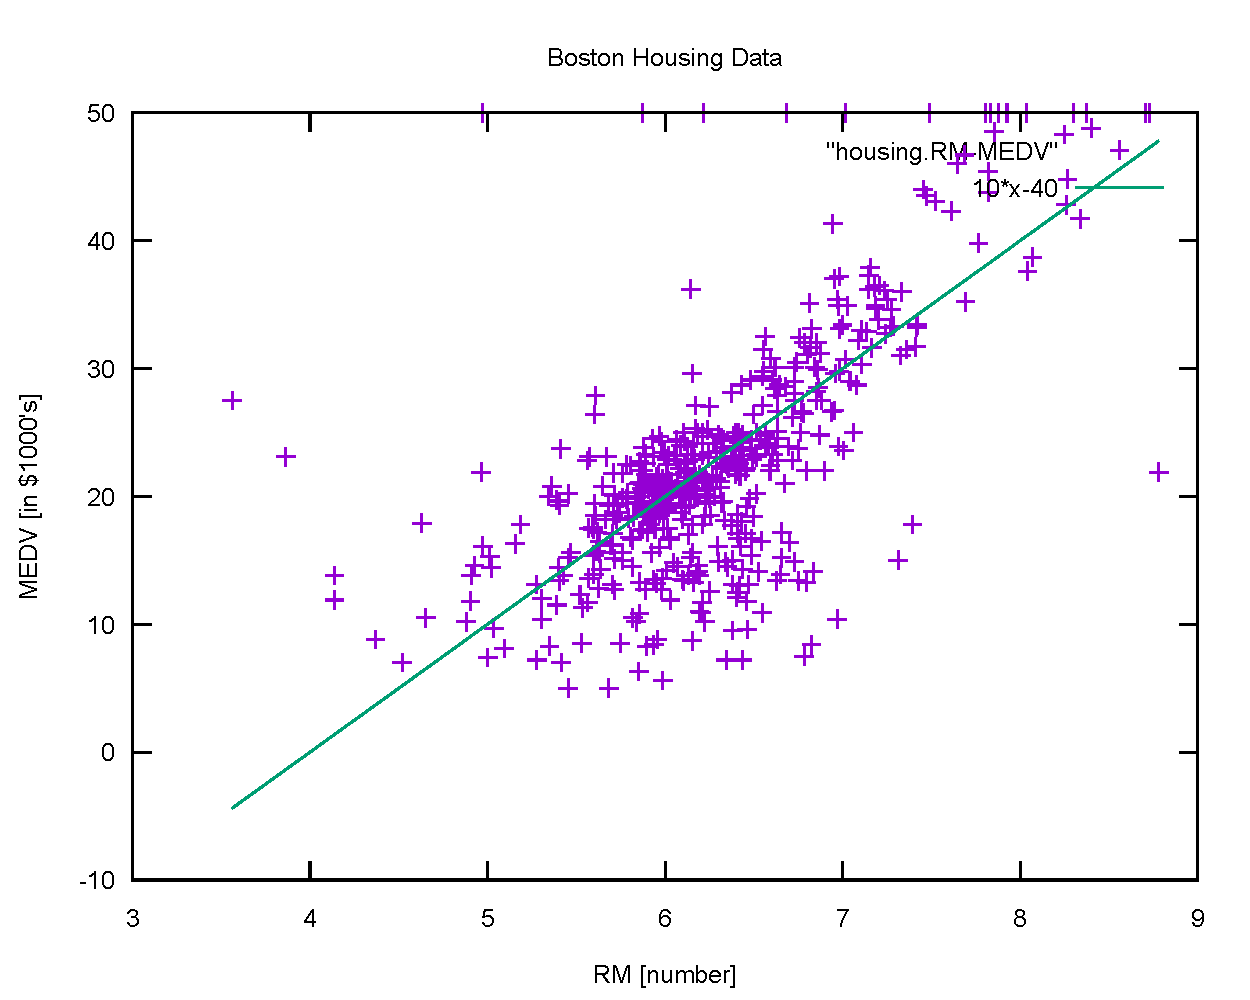
\includegraphics[width=10.0cm]{figs/level1.2/housing.pdf}
  \caption{探索初期値の変化}
 \end{center}
\end{figure}



